\documentclass[11pt, letterpaper]{article}

% -------------------------------------------------------------------------
% Commands
\usepackage[utf8]{inputenc}
\usepackage{graphicx}
\usepackage{hyperref}
\usepackage{cite}
\usepackage{vmargin}
\usepackage{lipsum}
\usepackage{amsmath}

\setmargins{2.5cm}                 % left margin
{1.5cm}                            % top margin
{16.5cm}                           % text width
{23.42cm}                          % text height
{10pt}                             % header height
{1cm}                              % space between text and headers
{0pt}                              % footer height
{2cm}                              % space between text and footer

% -------------------------------------------------------------------------
\title{\textbf{Modeling Auxotroph Growth}}

\date{}
\author{}

% -------------------------------------------------------------------------
% opening
\begin{document}

\maketitle

We are using an E.coli COBRA-like model as described in \cite{alterProteomeRegulationPatterns2021}, which is based on the \textbf{iML1515} network \cite{monkIML1515KnowledgebaseThat2017}. 
This model includes protein allocation constraints, so we refer to it as the \textbf{PAModel}.
We are introducing mutations to simulate specific auxotrophies:
i. $\Delta$\textit{Met}, in which the \textbf{HSST} reaction is knocked out, resulting in inability to grow without methionine;
ii. $\Delta$\textit{Ile}, in which the \textbf{THRD-L} reaction is knocked out, leading to an isoleucine auxotrophy.

For each auxotrophy, we perform an \textbf{FBA} simulation to evaluate the optimal growth rate, given defined maximal available glucose and essential amino acid intake rates, denoted as $U_{glc}$ and $U_{aa}$ respectively. Specifically, we maximize the objective function:

\[
10^{4}  \, q_{\text{growth rate}}
- 10^{0}  \, q_{glc}
- 10^{-2} \, q_{aa},
\]

where $q_{\text{growth rate}}$ is the growth rate, and $q_{glc}$ and $q_{aa}$ are the fluxes of intake for glucose and the essential aminoacid respectively. Note the difference between the bound $U_*$ and the flux $q_*$. The bound is a constraint on the flux. The flux is a free variable of the optimization problem. 


\begin{figure}[h!]
	\centering
	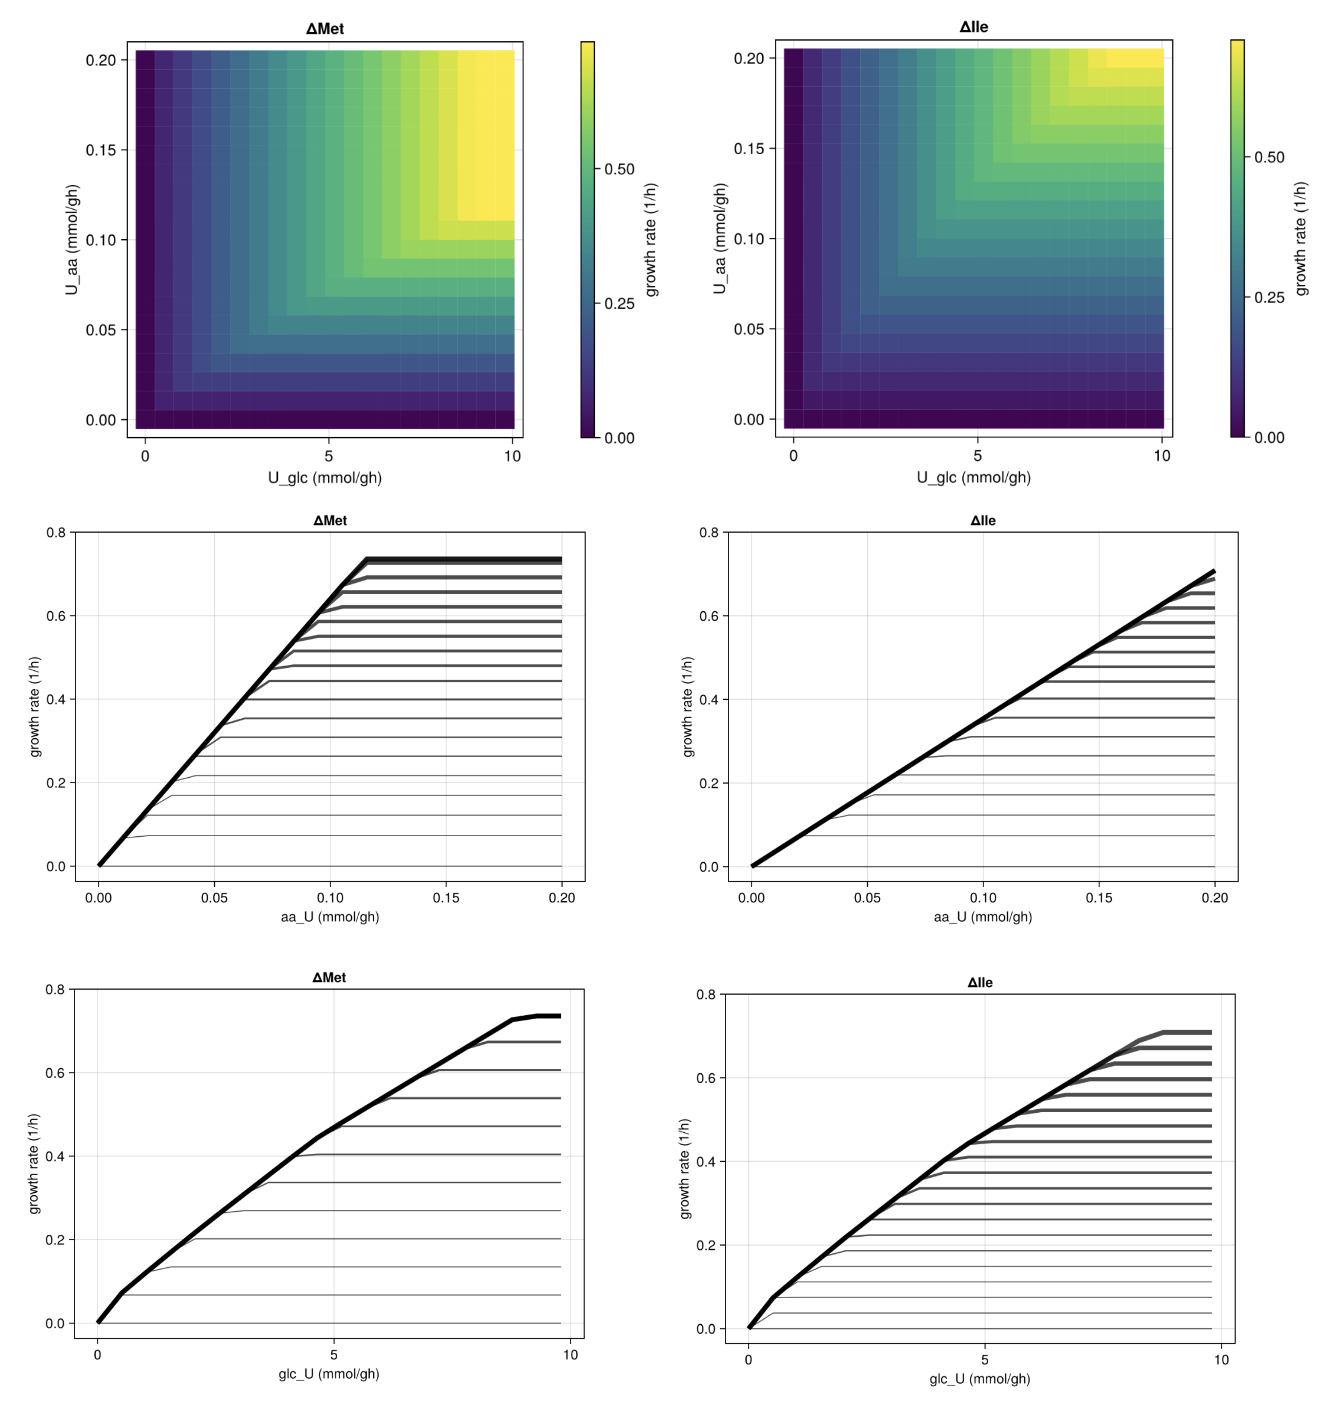
\includegraphics[scale = 0.65]{images/aa_U-glc_U-biom.png}
	\caption{
    \textbf{Row 1}: Heatmaps of optimal growth rate as a function of nutrient bounds.
    \textbf{Row 2}: Optimal growth rate as a function of essential amino acid bound at fixed glucose bound. Line width is proportional to the glucose bound.
    \textbf{Row 3}: Optimal growth rate as a function of glucose bound at fixed essential amino acid bound. Line width is proportional to the essential amino acid bound.
  }
	\label{fig:aa_U-glc_U-biom}
\end{figure}

Figure~\ref{fig:aa_U-glc_U-biom} shows results from these simulations. 
As expected for two non-substitutable nutrients with limited availability, increasing the growth rate eventually reaches a region where at least one nutrient becomes limiting.
This limiting status is identified by observing that the optimal growth rate is sensitive to further increases in nutrient availability.

In the case of the essential amino acids, the optimal solution uses them in a consistent manner, likely directly as precursors for biomass synthesis. 
This is suggested by the simple shape of the curves in row 2 of the figure, which show a region of constant slope (the amino acid-limited regime) followed by a flat region where glucose becomes the limiting nutrient.

For glucose, the picture is slightly more complex.
As shown in row 3 of the figure, the yield (i.e. the slope in the limiting region) depends on the glucose intake itself. 
This can be explained by the proteome allocation constraints, which depend on all fluxes, especially on the growth rate and nutrient uptake fluxes.

\bibliographystyle{plain}
\bibliography{main}
	
\end{document}

